\documentclass{ximera}
%% handout
%% nohints
%% space
%% newpage
%% numbers

%% You can put user macros here
%% However, you cannot make new environments

\graphicspath{{./}{firstExample/}{secondExample/}}

\usepackage{url}
\usepackage{tikz}
\usepackage{tkz-euclide}
\usetkzobj{all}


\tikzstyle geometryDiagrams=[ultra thick,color=blue!50!black]
\pgfplotsset{compat=1.8}
  \usepackage[T1]{fontenc}
  \usepackage[utf8x]{inputenc} %% we can turn off input when making a master document

\prerequisites{none}

\title{Transformations}

\begin{document}
\begin{abstract}
We learn how to find formulas that stretch and shift functions.
\end{abstract}
\maketitle

\subsection*{Basic learning objectives}

These are the tasks you should be able to perform with reasonable fluency \textbf{when you arrive at our next class meeting}. Important new vocabulary words are indicated \emph{in italics}. 

\begin{itemize}
	\item Know how to shift a function to the right by $h$ units or up by $k$ units.
	\item Know how to scale a function vertically by a factor of $a$ or horizontally by a factor of $b$.
	\item Be able to recognize all the parent functions from the previous two sections.
\end{itemize}

\subsection*{Advanced learning objectives}

In addition to mastering the basic objectives, here are the tasks you should be able to perform \textbf{after class, with practice}: 

\begin{itemize}
	\item Find the exact equation of a curve based on one of the parent functions.
    \item Understand how order matters when shifting and scaling functions.
    \item Be able to plot curves with a restricted domain and be able to draw a picture using \link{http://desmos.com}.
\end{itemize}

\noindent\hrulefill

Now that we have mastered the basic parent functions, we will use these parent functions as building blocks for other functions. We can transform the graph of a function by shifting the graph horizontally or vertically or by scaling (stretching) the graph horizontally or vertically. The rules are as follows.

\begin{itemize}
\item To shift $y=f(x)$ to the right by $h$ units we replace $x$ with $x-h$.
\item To shift $y=f(x)$ to up by $k$ units we replace $y$ with $y-k$.
\item To scale $y=f(x)$ horizontally by a factor of $b$ we replace $x$ with $\frac{1}{b} x$.
\item To scale $y=f(x)$ vertically by a factor of $a$ we replace $y$ with $\frac{1}{a} y$.
\end{itemize}

For example, suppose we want to scale the parabola $y=x^2$ vertically by a factor of $2$, and then shift the parabola $2$ units to the right and $3$ units down.

First replace $y$ with $\frac{1}{2}y$ to get $\frac{1}{2}y=x^2$. Then replace $x$ with $x-2$ and $y$ with $y+3$ to get 
\[\frac{1}{2}(y+3)=(x-2)^2.\] 
This answer is correct, though we typically solve for $y$ by multiplying both sides by $2$ and subtracting $3$ from both sides to get
\[
y=2(x-2)^2-3.
\]

Using function notation we can rewrite the $4$ rules for transforming functions as follows.

\begin{itemize}
\item To shift $y=f(x)$ to the right by $h$ units use $y=f(x-h)$.
\item To shift $y=f(x)$ to up by $k$ units use $y=f(x)+k$.
\item To scale $y=f(x)$ horizontally by a factor of $b$ use $y=f\left(\frac{1}{b}x\right)$.
\item To scale $y=f(x)$ vertically by a factor of $a$ use $y=a f(x)$.
\end{itemize}

\begin{question}
In \href{http://desmos.com}{http://desmos.com} plot the function $f(x)=x^2$. Then enter functions $y=af(x)$ and $y=f\left(\frac{1}{b}x\right)$ and create sliders for $a$ and $b$. Compare the graph when $b=\frac{1}{2}$ and $a=1$ with the graph when $a=4$ and $b=1$. Which statement accurately describes the relationship between the resulting graphs?

    \begin{multipleChoice}
      \choice[correct]{Scaling $y=x^2$ horizontally by a factor of $\frac{1}{2}$ is the same as scaling it vertically by a factor of $4$.}
      \choice{Scaling $y=x^2$ horizontally by a factor of $2$ is the same as scaling it vertically by a factor of $4$.}
      \choice{Scaling $y=x^2$ horizontally by a factor of $2$ is the same as scaling it vertically by a factor of $\frac{1}{4}$.}
      \choice{Scaling $y=x^2$ horizontally by a factor of $\frac{1}{2}$ is the same as scaling it vertically by a factor of $\frac{1}{4}$.}
    \end{multipleChoice}
    \begin{hint}
    Note that $4x^2=(2x)^2=\left(\frac{1}{1/2}x\right)^2$.
    \end{hint}
Which case below results in the narrowest graph?
	\begin{multipleChoice}
      \choice{$a=2$, $b=1$}
      \choice[correct]{$a=4$, $b=1$}
      \choice{$a=1$, $b=2$}
      \choice{$a=1$, $b=4$}
    \end{multipleChoice}
    
If the graph of the parabola $y=ax^2$ goes through the point $(3,1)$, then $a=$ \answer{1/9}. If the parabola $y=\left(\frac{1}{b}x\right)^2$ goes through the point $(3,1)$, then $b=$ \answer{1/3}.  
	\begin{hint}
    Use the sliders to find the values. Remember that you can narrow down the possible values for the parameters $a$ and $b$ by clicking below the sliders.
    \end{hint}

\end{question}

\begin{question}
In \link{http://desmos.com} plot the function $f(x)=2x$. Then enter functions $y=f(x-h)$ and $y=f(x)+k$ and create sliders for $h$ and $k$. Compare the graphs when $h=-1$ and $k=2$. Which statement accurately describes the relationship between the resulting graphs?

    \begin{multipleChoice}
      \choice[correct]{Shifting $y=2x$ horizontally by $-1$ unit is the same as shifting the graph vertically by $2$ units.}
      \choice{Shifting $y=2x$ horizontally by $1$ unit is the same as shifting the graph vertically by $2$ units.}
      \choice[correct]{Shifting $y=2x$ horizontally by $1$ unit is the same as shifting the graph vertically by $-2$ units.}
      \choice{Shifting $y=2x$ horizontally by $-1$ unit is the same as shifting the graph vertically by $-2$ units.}
    \end{multipleChoice}
    \begin{hint}
    Note that $2(x-(-1))=2x+2$.
    \end{hint}
If the graph of the line goes through the point $(2,0)$, then $h=$ \answer{2} or $k=$ \answer{-4}.  
	\begin{hint}
    Use the sliders to find the values. 
    \end{hint}

\end{question}

\begin{question}
Below is a transformation of the parent function $y=x^3$. 
\begin{image}
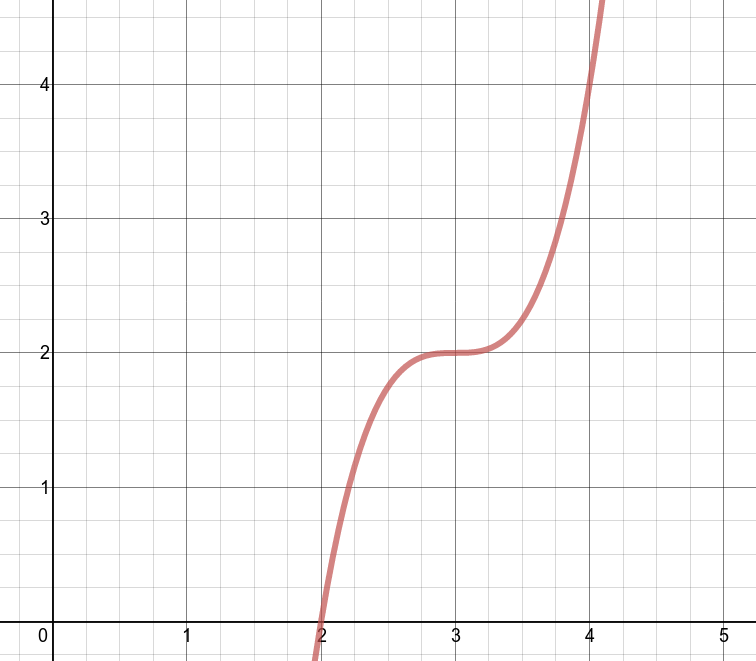
\includegraphics[width=6cm]{2_x-3_cubed+2.png}
\end{image}
The formula for this function can be written in the form $f(x)=a(x-h)^3+k$ where $a=$ \answer{2}, $h=$ \answer{3}, and $k=$ \answer{2}.
\end{question}

\begin{question}
Below is a transformation of the parent function $y=|x|$. 
\begin{image}
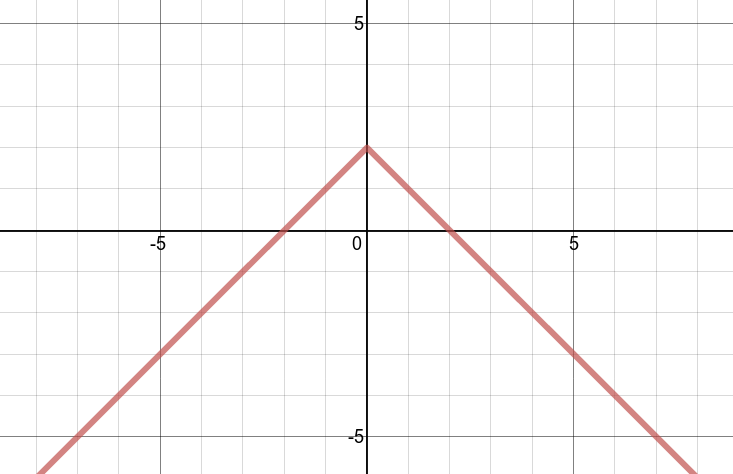
\includegraphics[width=8cm]{neg_x_+2.png}
\end{image}
The formula for this function can be written in the form $f(x)=a|x-h|+k$ where $a=$ \answer{-1}, $h=$ \answer{0}, and $k=$ \answer{2}.
\end{question}



\end{document}
